% Chapter 2

\chapter{\uppercase{FUNDAMENTALS OF THE DETECTION OF ANOMALIES}}

\label{Capitulo 2}

This chapter discusses necessary concepts that are needed to understand the detection of anomalies, as well as different projects and investigations carried out in field of the detection of driving anomalies to date.
%En este cap\'{i}tulo se aborda los conceptos necesarios que se necesita para comprender la detecci\'{o}n de anomal\'{i}as, as\'{i} tambi\'{e}n se expone los diferentes proyectos e investigaciones realizados en el campo de la detecci\'{o}n de anomal\'{i}as de conducci\'{o}n hasta la fecha.

\section{Anomaly detection}

To understand what anomaly detection implies, it is necessary to assimilate what an anomaly is, and in what ways these can occur. Therefore, it can be said that anomalies, or outliers, are patterns in the data that do not fit a well-defined notion of normal behavior.
%Para comprender lo que implica la detecci\'{o}n de anomal\'{i}as, es necesario asimilar lo que \'{e}s una anomal\'{i}a, y de qu\'{e} maneras \'{e}stas pueden presentarse. Por lo tanto, se puede decir que las \textbf{anomalías}, o valores at\'{i}picos, son patrones en los datos que no se ajustan a una noción bien definida de un comportamiento normal.

\vspace{5mm} %5mm vertical space

Anomalies can be classified into one of the following three categories:
%Las anomal\'{i}as pueden ser clasificadas dentro de una de las tres siguientes categor\'{i}as:

\begin{enumerate}[1.]

\item \textbf{Point anomalies: }Point anomalies are simply unique and anomalous instances within a larger data set, that is, they are separated from the rest of the data. For example, in Figure \ref{fig:anom_2D}, points $o_1$, $o_2$ and region $O_3$ are outside the limits of normal regions ($N_1$ and $N_2$), and therefore are point anomalies because they are different from the normal data set.

%\item \textbf{Anomal\'{i}as de punto: }Las anomalías de punto son simplemente instancias únicas y anómalas dentro de un conjunto de datos más grande, es decir, \'{e}stas se encuentran separadas del resto de los datos. Por ejemplo, en la Figura \ref{fig:anom_2D}, los puntos $o_1$, $o_2$ y la regi\'{o}n $O_3$ se encuentran fuera de los l\'{i}mites de las regiones normales ($N_1$ y $N_2$), y por lo tanto son anomal\'{i}as puntuales debido a que son diferentes al conjunto de datos normales.

\begin{figure}[h!]
  \begin{center}	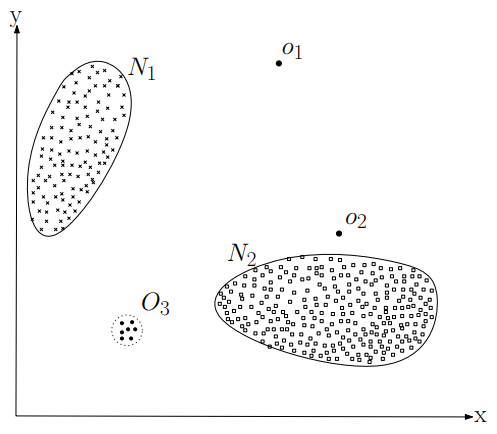
\includegraphics[width=0.45\textwidth,frame]{imagenes/Cap2/anom_2D}
  \caption{Example of point anomalies in a 2-dimensional data set \protect\cite{Reference66}.}
  \label{fig:anom_2D}
  \end{center}
\end{figure}

\vspace{5mm} %5mm vertical space

This type of anomaly is considered the simplest and is the focus of most research focused on anomaly detection.
%Este tipo de anomal\'{i}a se considera la m\'{a}s simple y es el foco de la mayor\'{i}a de las investigaciones enfocadas en la detecci\'{o}n de valores at\'{i}picos.

\item \textbf{Contextual (or conditional) anomalies: }These are points that are only considered anomalous in a specific context. The notion of this context is induced by the structure in the data set and must be specified as part of the problem formulation.
%\item \textbf{Anomal\'{i}as contextuales (o condicionales): }Estos son puntos que s\'{o}lo se consideran anómalos en un contexto espec\'{i}fico. La noci\'{o}n de este contexto es inducida por la estructura en el conjunto de datos y debe especificarse como parte de la formulaci\'{o}n del problema.

\vspace{5mm} %5mm vertical space

These types of anomalies have been explored more frequently in time series and spatial data. Figure \ref{fig:anom_contx} shows an example of a time series of the monthly temperature of an area in the last 5 years, it should be taken into account that the temperature at time $t_1$ is the same as at time $t_2$, but occurs in a different context , therefore $t_2$ is considered an anomaly.
%Este tipo de anomal\'{i}as se han explorado con mayor frecuencia en los datos de series de tiempo y datos espaciales. La figura \ref{fig:anom_contx} muestra un ejemplo de serie temporal de la temperatura mensual de un \'{a}rea en los \'{u}ltimos 5 a\~{n}os, se debe tener en cuenta que la temperatura en el tiempo $t_1$ es la misma que en el tiempo $t_2$, pero se produce en un contexto diferente, por lo tanto $t_2$ es considerada una anomal\'{i}a.

\begin{figure}[h!]
  \begin{center}	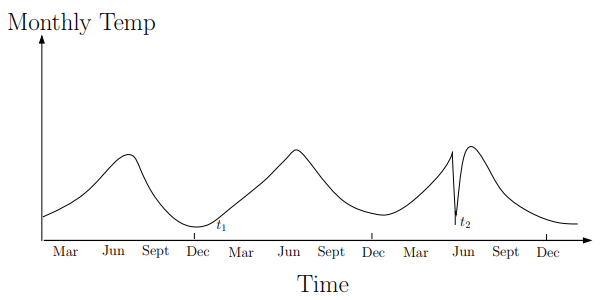
\includegraphics[width=0.6\textwidth,frame]{imagenes/Cap2/anom_contx}
  \caption{Contextual anomaly $t_2$ in a temperature time serie \protect\cite{Reference66}.}
  \label{fig:anom_contx}
  \end{center}
\end{figure}

\item \textbf{Collective anomalies: } If a collection of related data instances is anomalous with respect to the entire data set, it is called a collective anomaly. The instances of individual data in a collective anomaly may not be anomalies by themselves, but their joint appearance as a collection is anomalous.
%\item \textbf{Anomal\'{i}as colectivas: } Si una colección de instancias de datos relacionadas es anómala con respecto a todo el conjunto de datos, se denomina anomalía colectiva.  Las instancias de datos individuales en una anomalía colectiva pueden no ser anomalías por sí mismas, pero su aparición conjunta como una colección es anómala.

\vspace{5mm} %5mm vertical space

Figure \ref{fig:anom_col} illustrates an example showing a human electrocardiogram output, it can be noted that the region highlighted in red denotes an anomaly because there is the same low value for an abnormally long time (corresponding to a premature atrial contraction). It should be taken into account that this low value by itself is not considered an anomaly.
%La figura \ref{fig:anom_col} ilustra un ejemplo que muestra una salida de electrocardiograma humano, se puede notar que la región resaltada en rojo denota una anomalía porque existe el mismo valor bajo durante un tiempo anormalmente prolongado (que corresponde a una Contracción prematura auricular). Se debe tener en cuenta que ese valor bajo por sí mismo no es considerada una anomalía.

\begin{figure}[h!]
  \begin{center}	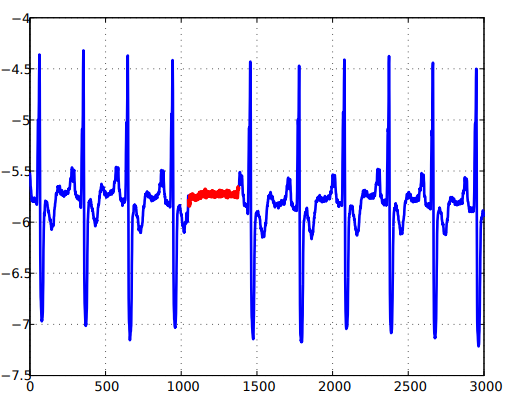
\includegraphics[width=0.45\textwidth,frame]{imagenes/Cap2/anom_col}
  \caption{Collective anomaly corresponding to premature atrial contraction in a human electrocardiogram \protect\cite{Reference66}.}
  \label{fig:anom_col}
  \end{center}
\end{figure}

\end{enumerate}

In relation to the above, it can be defined as detection of anomalies, or outliers, to the identification of data points, elements, observations or events that do not fit the expected pattern of a particular group.
%En relaci\'{o}n a lo expuesto previamente se puede definir como \textbf{detecci\'{o}n de anomal\'{i}as}, \'{o} \textbf{valores at\'{i}picos}, a la identificación de puntos de datos, elementos, observaciones o eventos que no se ajustan al patrón esperado de un grupo determinado. 

\vspace{5mm} %5mm vertical space

Anomaly detection is used in different application domains, for example: image processing, card fraud detection, network intrusion detection systems, etc.
%La detecci\'{o}n de anomal\'{i}as, se usa en distintos dominios de aplicaciones, por ejemplo: procesamiento de im\'{a}genes, detecci\'{o}n de fraudes de tarjeta, sistemas de detecci\'{o}n de intrusi\'{o}n de red, \'{e}tcetera.

\section{Challenges in anomaly detection}

On an abstract level, anomaly detection may seem like a simple task. However, it can be a very challenging task. Below are some of these challenges.
%En un nivel abstracto, la detecci\'{o}n de anomal\'{i}as puede parecer una tarea simple. Sin embargo puede llegar a ser una tarea muy desafiante. A continuaci\'{o}n se presenta algunos de estos desaf\'{i}os.

\begin{itemize}
\item The definition of normal regions is quite difficult. In many cases, the boundaries between anomalies and normal data are not accurate. Therefore, normal observations could be considered anomalies and vice versa.
%\item La definici\'{o}n de regiones normales es bastante dif\'{i}cil. En muchos casos, los l\'{i}mites entre las anomal\'{i}as y los datos normales no son precisos. Por lo tanto, las observaciones normales podr\'{i}an considerarse anomal\'{i}as y viceversa.

\item Therefore, normal observations could be considered anomalies and vice versa.
%\item Lo que se considera normal hoy en d\'{i}a, puede no ser normal en el futuro.

\item Most of the time the approaches for detecting anomalies in a specific field cannot be used in another field.
%\item La mayor parte de las veces los enfoques para la detecci\'{o}n de anomal\'{i}as en un campo en espec\'{i}fico no se pueden utilizar en otro campo.

\item The low availability of positive samples (anomalies) for training and validation of anomaly detection model.
%\item La poca disponibilidad de ejemplos positivos (anomal\'{i}as) para el entrenamiento y validaci\'{o}n del modelo de detecci\'{o}n de anomal\'{i}as.

\end{itemize}

\subsection{Anomaly detection approaches}

The approaches that can be used for this purpose are classified into following categories:
%Los enfoques que se pueden usar para este prop\'{o}sito se clasifican en las siguientes categor\'{i}as:

\subsubsection{Supervised anomaly detection}

The use of supervised learning techniques requires the availability of a set of labeled training data, for both normal and anomalous classes. The main focus is to build a predictive model for normal classes vs. anomalies, then take any instance of unseen data, compare with model and determine to which class it belongs.
%El uso de t\'{e}cnicas de aprendizaje supervisado requiere la disponibilidad de un conjunto de datos de entrenamiento etiquetados, tanto para clases normales como an\'{o}malas. El enfoque principal es construir un modelo predictivo para clases normales vs. anomal\'{i}as, posteriormente tomar cualquier instancia de datos no visto, comparar con el modelo y determinar a que clase pertenece.

\vspace{5mm} %5mm vertical space

There are two main drawbacks that arise with the use of this technique.
%Existen dos principales inconvenientes que surgen con el uso de \'{e}sta t\'{e}cnica.

\begin{itemize}

\item The number of anomalous instances is much lower than that of the normal instances, which creates an imbalance of class distribution during training.
%\item La cantidad de instancias an\'{o}malas es muy inferior a la de las instancias normales, lo que genera un desequilibrio de distribuci\'{o}n de clases durante el entrenamiento.
\item Obtaining accurate and representative labels, particularly for anomaly class, is a challenge.
%\item La obtenci\'{o}n de etiquetas precisas y representativas, en particular para la clase de anomal\'{i}a, es un desaf\'{i}o.
\end{itemize}

\subsubsection{Semi-supervised anomaly detection}

These techniques require a training set with labeled instances, but only for the normal class, this makes its use more applicable than the supervised techniques, since no labels are required for the anomaly class.
%Estas t\'{e}cnicas requieren un conjunto de entrenamiento con instancias etiquetadas, pero solo para la clase normal, esto hace que su uso sea m\'{a}s aplicable que las t\'{e}cnicas supervisadas, ya que no se requiere etiquetas para la clase anomal\'{i}a.

\vspace{5mm} %5mm vertical space

The typical approach used in these techniques is to build a model for the class corresponding to normal behavior, and use model to identify anomalies in the test data.
%El enfoque típico usado en \'{e}stas técnicas es construir un modelo para la clase correspondiente al comportamiento normal, y usar el modelo para identificar anomalías en los datos de prueba.

\subsubsection{Unsupervised anomaly detection}

Techniques that operate in an unsupervised manner do not require training data, which is why they are the most widely used. These techniques assume that normal instances are much more frequent than anomalies in test data, in case this assumption is not true, such techniques suffer from a high rate of false alarms.
%Las t\'{e}cnicas que operan de manera no supervisada no requieren datos de entrenamiento, raz\'{o}n por la cual son las m\'{a}s ampliamente utilizadas. Estas t\'{e}cnicas suponen que las instancias normales son mucho m\'{a}s frecuentes que  las anomal\'{i}as en los datos de prueba, en caso de que esta suposici\'{o}n no sea cierta, tales t\'{e}cnicas sufren de una alta tasa de falsas alarmas.

\section{Related work}

The identification of abnormal driving behaviors is an indispensable part of improving driving safety, however, as previously described, this is not a simple task. In recent years, several techniques have been proposed to detect driving behaviors. This section is dedicated to review them.
%La identificación de comportamientos de conducción anormal es una parte indispensable para mejorar la seguridad de conducción, sin embargo, como se describi\'{o} previamente, \'{e}sta no es una tarea sencilla. En los últimos años, se han propuesto varias técnicas para detectar conductas de conducci\'{o}n. Esta secci\'{o}n esta dedicada al repaso de las mismas.

\vspace{5mm} %5mm vertical space

\shortciteA{Reference20}, propose a combined system that consists of two modules: one to detect the type of vehicle of users and the other to detect events of instant driving, regardless of the orientation and position of smartphones, this system It achieves an average accuracy of 98.33\% in detection of vehicles's type (car, motorcycle, bicycle, among others) and an average accuracy of 98.95\% in recognition of motorcyclist driving events when using Random Forest as a classifier.
%\shortciteA{Reference20}, proponen un sistema combinado que se compone de dos módulos: uno para detectar el tipo de vehículo de los usuarios y el otro para detectar los eventos de conducción instantánea, independientemente de la orientación y la posición de los teléfonos inteligentes, \'{e}ste sistema logra una precisión promedio del 98.33\% en la detección del tipo del vehículo (autom\'{o}vil, motocicleta, bicicleta, entre otros) y una precisión promedio de 98.95\% en el reconocimiento de los eventos de conducción de los motociclistas al usar Random Forest como clasificador.

\vspace{5mm} %5mm vertical space

On the other hand \shortciteA{Reference21} present a quantitative evaluation of 4 Machine Learning algorithms (Bayesian Network BN, Artificial Neural Network ANN, Random Forest RF and Support Vector Machine SVM) with different configurations, applied in the detection of 7 types of driving events, between events normal and aggressive, using data collected from 4 Android smartphone sensors (accelerometer, linear acceleration, magnetometer and gyroscope); resulting in the gyroscope and accelerometer being the best sensors to detect driving events and that Random Forest (RF) is by far the best-performing Machine Learning Algorithm, followed by the simplest form of ANN the Multi Layer Perceptron ( MLP).
%Por otra parte \shortciteA{Reference21} presentan una evaluación cuantitativa de 4 algoritmos de Aprendizaje Autom\'{a}tico ( Bayesian Network BN, Artificial Neural Network ANN, Random Forest RF y Support Vector Machine SVM) con diferentes configuraciones, aplicadas en la detección de 7 tipos de eventos de conducción, entre eventos normales y agresivos, utilizando datos recopilados de 4 sensores de teléfonos inteligentes Android (acelerómetro, aceleración lineal, magnetómetro y giroscopio); dando como resultado que el giroscopio y el acelerómetro son los mejores sensores para detectar eventos de conducción y que Random Forest (RF) es por lejos el Algoritmo de Aprendizaje Autom\'{a}tico de mejor rendimiento, seguido de la forma m\'{a}s simple de ANN el Multi Layer Perceptron (MLP).

\vspace{5mm} %5mm vertical space

\citeA{Reference23} propose the MIROAD system which shows that Dynamic Time Warping (DTW) is a valid algorithm to detect potentially aggressive driving maneuvers, where almost all aggressive events (97\%) were correctly identified, using the set of T sensors (accelerometer, gyroscope and tone of voice). Likewise, in the work of Kridalukmana, Yan-Lu, and Naderpour (2017), a system focused on developing driver awareness through notifications in critical situations that can trigger unsafe driving maneuvers is proposed, using a model to detect dangerous situations based on Object-Oriented Bayesian Network (OOBN).
%\citeA{Reference23} proponen el sistema MIROAD el cual muestra que el Dynamic Time Warping (DTW) es un algoritmo válido para detectar maniobras de conducción potencialmente agresivas, donde casi todos los eventos agresivos (97\%) se identificaron correctamente, utilizando el conjunto de sensores T (aceler\'{o}metro, giroscopio y el tono de voz). As\'{i} tambi\'{e}n en el trabajo de \citeA{Reference24} se propone un sistema enfocado a desarrollar la conciencia del conductor mediante notificaciones en situaciones críticas que pueden desencadenar maniobras de conducci\'{o}n inseguras, mediante un modelo para detectar situaciones peligrosas basadas en Object-Oriented Bayesian Network (OOBN).

\vspace{5mm} %5mm vertical space

As well as the works presented previously there is a large number of works (\citeNP{Reference25}; \citeNP{Reference26}; \citeNP{Reference27}; \citeNP{Reference28}; \citeNP{Reference29}) that use smart phone sensors (accelerometer and gyroscope) for aggressive driving detection, due of advantage of not buying or installing any device and besides being highly portable, however it depends a lot on the performance of GPS receiver and is not applicable in areas not available for GPS.
%As\'{i} como los trabajos presentados previamente existe gran cantidad de trabajos (\citeNP{Reference25}; \citeNP{Reference26}; \citeNP{Reference27}; \citeNP{Reference28}; \citeNP{Reference29}) que usan los sensores de los tel\'{e}fonos inteligentes (aceler\'{o}metro y giroscopio) para la detecci\'{o}n de conducci\'{o}n agresiva, esto debido a que se tiene la ventaja de no comprar ni instalar ning\'{u}n dispositivo y adem\'{a}s de ser altamente port\'{a}til, sin embargo se depende bastante del rendimiento del receptor GPS y no es aplicable en \'{a}reas no disponibles para GPS.

\vspace{5mm} %5mm vertical space

There are also other approaches to detection of aggressive driving of a driver, for instance in the work of \citeA{Reference22}, a method based on Convolutional Neural Network (CNN) is proposed) to detect the emotion of aggressive driving, by using a driver's facial images obtained with a NIR light camera and a thermal camera.
%Existen adem\'{a}s otros enfoques para la detecci\'{o}n de conducci\'{o}n agresiva de un conductor, por ejemplo en el trabajo de \citeA{Reference22} se propone un método basado en Convolutional Neural Network (CNN) para detectar la emoción de conducción agresiva, mediante la utilizaci\'{o}n de imágenes faciales de un conductor obtenidas con una cámara de luz NIR y una cámara térmica.

\section{Focus on the problem}

It is clear that this topic was extensively researched and that it has a wide variety of solution proposals, however most of these are based on detection by supervised learning techniques, which presents the great disadvantage of requiring data labeled to generate the model detection; In addition, much of related work proposes generalized models for detection and not specific models for each agent, which is crucial because each agent has individual driving behaviors and different conditions driving, that is, the driving of an agent that circulates through paved avenues will be different from driving of an agent that circulates through cobbled streets or driving of an agent that circulates through avenues or busy streets will be different from that of the agents that circulate through relatively decongested streets.
%Es evidente que \'{e}ste tema fue ampliamente investigado y que tiene una gran variedad de propuestas de soluci\'{o}n, sin embargo la mayor\'{i}a de estas se basan en la detecci\'{o}n mediante t\'{e}cnicas de aprendizaje supervisado, lo cual presenta la gran desventaja de requerir datos etiquetados para generar el modelo de detecci\'{o}n; adem\'{a}s gran parte de los trabajos relacionados proponen modelos generalizados para la detecci\'{o}n y no as\'{i} modelos espec\'{i}ficos por cada agente, lo cual es crucial debido a que cada agente presenta conductas individuales de conducci\'{o}n y conducen en condiciones distintas, es decir, la conducci\'{o}n de un agente que circula por avenidas pavimentadas ser\'{a} distinta a la conducci\'{o}n de un agente que circula por calles empedradas o la conducci\'{o}n de un agente que circula por avenidas o calles concurridas ser\'{a} distinta a de los agentes que circulen por calles relativamente descongestionadas.

\vspace{5mm} %5mm vertical space

The proposal made in this work is intended to provide a prototype of a tool that helps analyze the sequences of motion sensors of a mobile device and allows detecting anomalies from information obtained from this analysis.
%Con la propuesta que se hace en este trabajo se pretende brindar un prototipo de una herramienta que ayude a analizar las secuencias de los sensores de movimiento de un dispositivo m\'{o}vil y permita detectar anomalías a partir de la información obtenida de este análisis. 

\vspace{5mm} %5mm vertical space

To achieve this goal, the data set of motion sensors of a smartphone is captured, using a mobile application, then data is divided and prepared with data pre-processing techniques. Once these phases are completed, a model is trained with the training set and validated with the development set. Finally, an optimal model and a technique are chosen to classify outliers, in order to cover a full range of normal behaviors and exclude anomalies as accurately as possible. This method can best be seen in Figure \ref{fig:modeloAnomalias}.
%Para lograr este objetivo, se captura el conjunto de datos de los sensores de movimiento de un tel\'{e}fono inteligente, mediante una aplicaci\'{o}n m\'{o}vil, posteriormente se divide y prepara los datos con t\'{e}cnicas de pre-procesamiento de datos. Una vez terminadas estas fases se entrena un modelo con el conjunto de entrenamiento y se valida con el conjunto de desarrollo. Finalmente se elige un modelo \'{o}ptimo y una t\'{e}cnica para clasificar los valores at\'{i}picos, con el objetivo de cubrir un rango completo de los comportamientos normales y excluir con la mayor precisi\'{o}n posible las anomal\'{i}as. Este m\'{e}todo se puede apreciar mejor en la Figura \ref{fig:modeloAnomalias}.

\begin{figure}[h!]
  \begin{center}	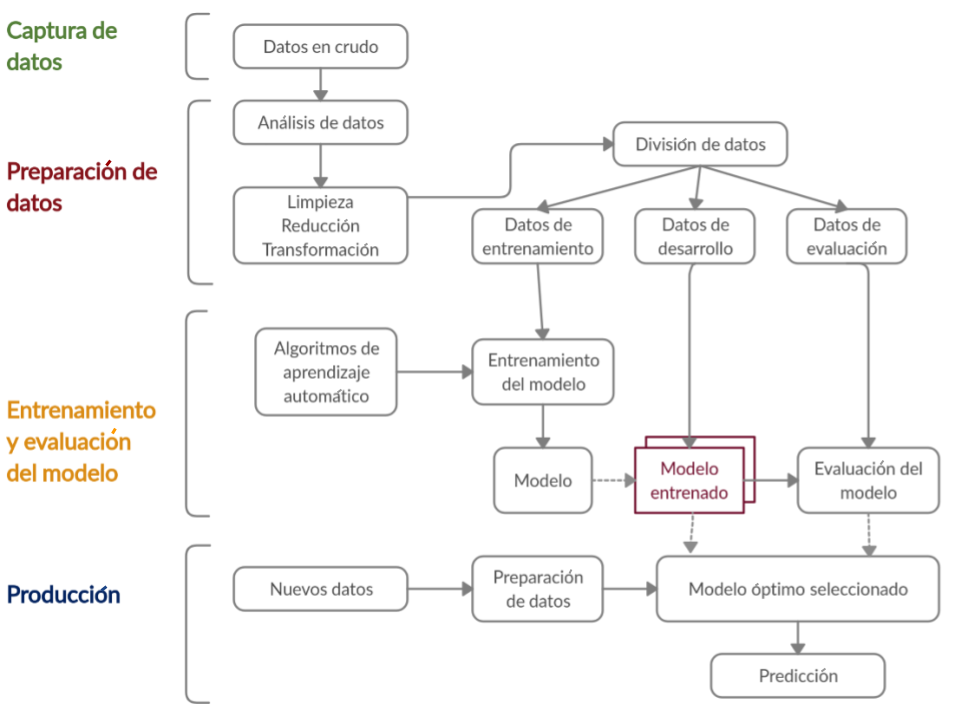
\includegraphics[width=0.90\textwidth,frame]{imagenes/Cap2/metodo1}
  \caption{Proposed anomaly detection method (Own elaboration).}
  \label{fig:modeloAnomalias}
  \end{center}
\end{figure}
%https://app.creately.com/diagram/XJJlVcfuoWy/view

%\section{Resumen del cap\'{i}tulo}

%De acuerdo a los conceptos presentados acerca de la detecci\'{o}n de anomal\'{i}as, los desaf\'{i}os  que presenta la detecci\'{o}n de las mismas y los trabajos de investigaci\'{o}n realizados en este campo hasta la fecha, se propone un m\'{e}todo de detecci\'{o}n de anomal\'{i}as de conducci\'{o}n mediante el uso de t\'{e}cnicas de Aprendizaje Autom\'{a}tico y el uso de un dispositivo m\'{o}vil, los mismos ser\'{a}n tratados en profundidad en los siguientes cap\'{i}tulos.